\begin{section}{Results}


\begin{frame}{Results (preliminary): Path Shape}
\begin{figure}
\begin{columns}[T,onlytextwidth]
\column{0.33\textwidth}
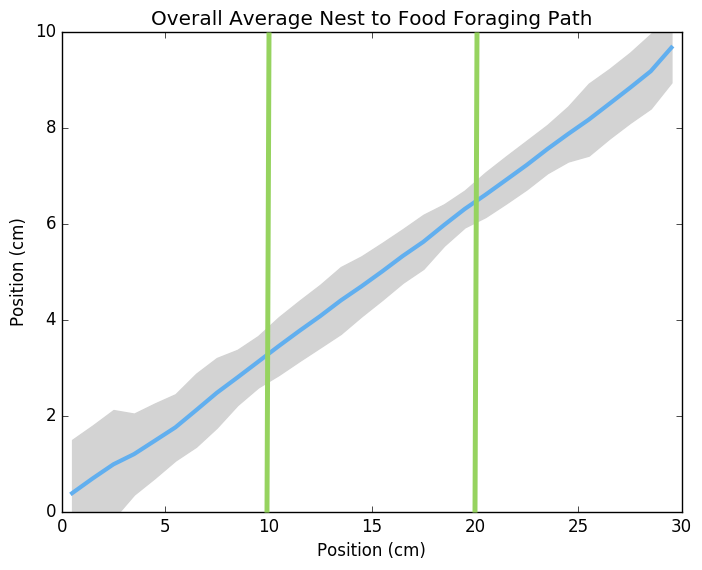
\includegraphics[width=\textwidth]{results/corner-to-corner-average_path_negpidiv3.png}
\column{0.005\textwidth}
\column{0.33\textwidth}
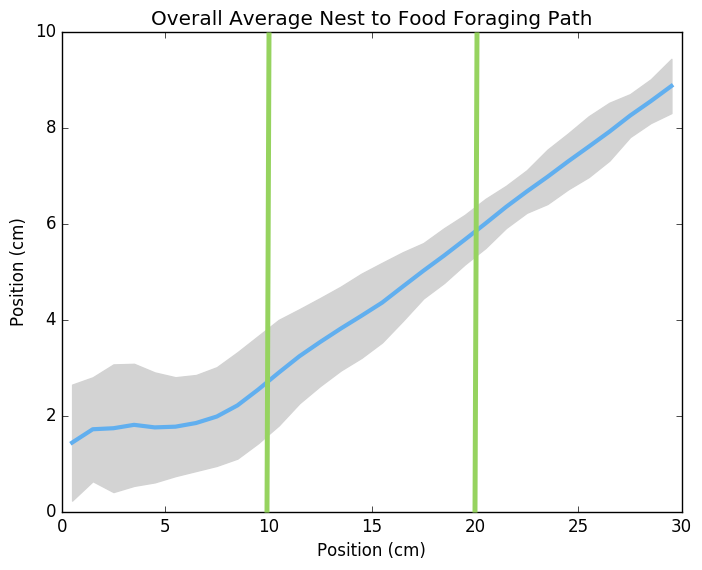
\includegraphics[width=\textwidth]{results/corner-to-corner-average_path_0.png}
\column{0.005\textwidth}
\column{0.33\textwidth}
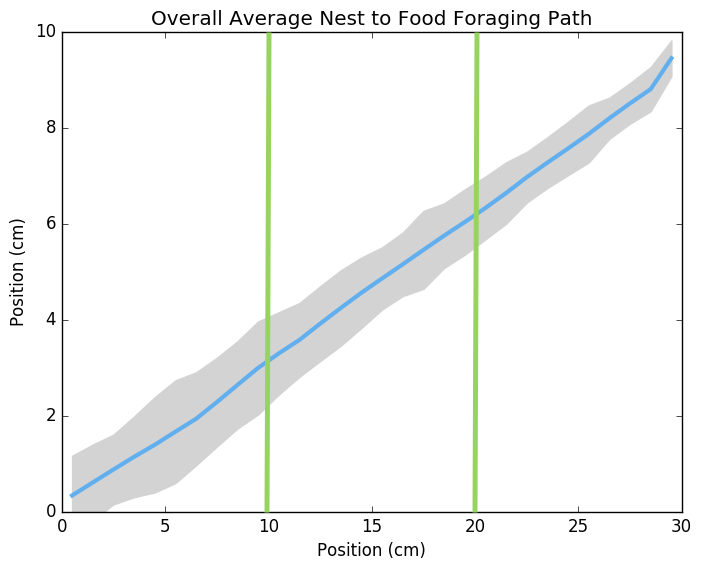
\includegraphics[width=\textwidth]{results/corner-to-corner-average_path_pidiv3.png}
\end{columns}
\caption{Comparison of overall average nest to food foraging path for, left to right, $-\pi/3$, $0$, and $\pi/3$ radian inclines.}
\end{figure}
\end{frame}


\begin{frame}{Results (preliminary): Path Length}
\begin{figure}
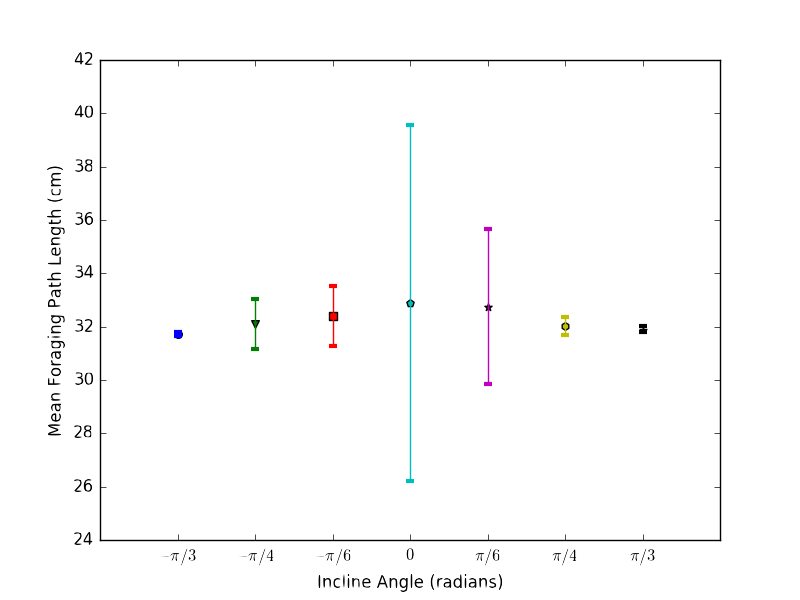
\includegraphics[width=0.8\textwidth]{results/corner-to-cornermeanforagingpathlength.png}
\caption{Comparison of path lengths over incline angles for corner-to-corner trials}
\end{figure}
\end{frame}

\begin{frame}{Results (preliminary): Trip Duration}
\begin{figure}
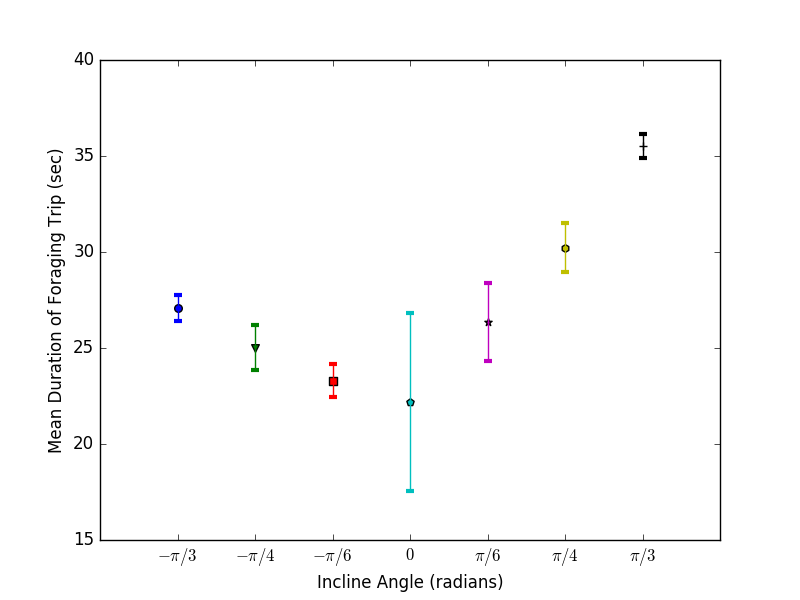
\includegraphics[width=0.8\textwidth]{results/corner-to-cornermeandurationofforagingtrip.png}
\caption{Comparison of trip durations over incline angles for corner-to-corner trials}
\end{figure}
\end{frame}


\begin{frame}{Next Steps}
\begin{columns}[T,onlytextwidth]
\column{0.5\textwidth}
\begin{itemize}
\item Refine model
	\begin{itemize}
		\item variable pheromone deposition rate
	\end{itemize}
\item Perform further sensitivity analyses
	\begin{itemize}
		\item pheromone grid granularity
        \item pheromone sensitivity radius of ant
        \item behavioral weighting
	\end{itemize}
%\item Perform replicate simulations
%\item Explore further combinations of experimental conditions
% \item More sophisticated analysis of ant paths (Splines?)
\item \textbf{Compare model predictions with empirical results}
\end{itemize}
\column{0.1\textwidth}
\column{0.4\textwidth}
\begin{figure}
        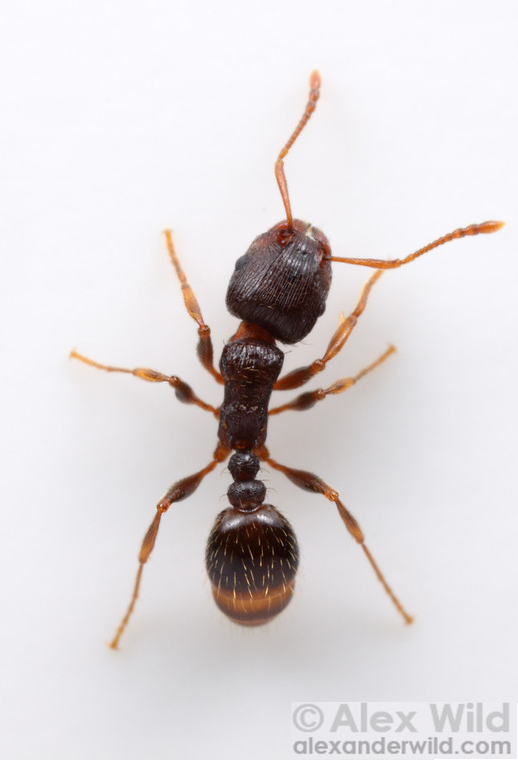
\includegraphics[width=\textwidth]{images/spE2-XL}
        \caption{\textit{Tetramorium caespitum} \scriptsize{\cite{spE2-XL.jpg_????}}}
\end{figure}
\end{columns}
\end{frame}


% \begin{frame}{Results (preliminary): Summary}
% \begin{itemize}
% 	\item as expected, foraging trips take longer over steeper incline and decline
% 	\begin{itemize}
% 		\item also taking longer over uphill versus downhill inclines
% 	\end{itemize}
% 	\vspace{1em}

% 	\item the foraging path is generally more stable with steep incline or decline
% 	\begin{itemize}
% 		%\item path is smoother
% 		\item ants are less likely to get lost/stuck
% 		\item this effect is less pronounced in the center-to-center arena
% 	\end{itemize}
% 	\vspace{1em}

% 	\item the foraging path becomes more direct with steeper incline or decline
% 	\vspace{-1em}
% 	\begin{itemize}
% 		\item even though the direct path is not aligned with the incline in the corner-to-corner arena
% 		\item this effect is less pronounced in the center-to-center arena
% 	\end{itemize}
% \end{itemize}
% \end{frame}

\end{section}